%
%
%

\chapter{Root Locus}\label{RootLocusChapter}

\section{Problem Statement and Learning Objectives}

Be able to
\begin{itemize}

  \item Explain the significance and identify the parts of a Root Locus diagram.
  \item Use the computer to plot Root Locus diagrams
  \item Hand draw  a Root Locus diagram for a given open-loop  transfer
  function (for positive gains  $k>0$ using the first 5 rules.
\end{itemize}





%%%%** Section 1.7
\section{Introduction to Root Locus}

In Section \ref{calculationofroots}, we examined roots of the characteristic polynomial of a closed loop negative feedback system (Figure \ref{openloopstable}) as a gain, $K$ was varied in increasing values from zero.    Root locus (invented by Walter Evans in 1948) is a graphical method to visualize the movement of poles of the closed loop system as gain is increased.   Since the location of the poles determine the stability  and step response dynamics, the root locus is extremely useful for design.

Back in 1948 it was very labor intensive to compute roots of a polynomial, especially to do it over and over for every value of $K$.   Like the BAMP, the Root Locus plot can be sketched by hand (with practice it becomes quick) and significant insights are gained.   As with BAMP, precise Root Locus diagrams are quickly obtained by computer so we don't have to worry about precision and detail in our hand sketch.









\subsection{Problem Definition}
What problem is Root Locus trying to solve? Consider the simple system of Figure \ref{simpleRLsystem}. There is one unknown parameter $K$ which we will assume is positive and real which represents a design parameter.  Up until now, we have mostly focused on analysis of existing systems.  Here we have the chance to design our system response (closed loop gain pole locations) by choosing our parameter $K$.

\begin{figure}\centering

%%%%%%%%%%%%%%%%%%%%%%%%%%%%%%%%%%%%%%%%%%%%%%%%%%%%%%%%%%%%%%%%%%%%%%%%%%%%%%%%%%%%%%%%

%        Closed loop control system

%%%%%%%%%%%%%%%%%%%%%%%%%%%%%%%%%%%%%%%%%%%%%%%%%%%%%%%%%%%%%%%%%%%%%%%%%%%%%%%%%%%%%%%%

\begin{tikzpicture}[every node/.style={draw, thick,outer sep=0pt,thick}]

% %
% debugging grid
%  \draw[step=5mm,gray,very thin] (-25mm,-25mm) grid (100mm,50mm);
%  \draw[thick,gray] (0,-25mm) -- (0,50mm);
%  \draw[thick,gray] (-25mm,0) -- (100mm,0);
%
%
%

 \node (C) [thick,minimum width=14mm, minimum height=10mm] {$\frac{K}{(s+3)}$};
 \node (H) [thick, yshift=-10mm] {$1$};

 \coordinate (outend) at ($(C.east)+(12.5mm,0)$);
 \coordinate (out2)   at ($(C.east)+(5mm,0)$);
 \draw [->] (C.east) -- (outend);
 \draw [->]  (out2)   -- ++(0,-10mm) -- (H.east);

 \node (sum)   [circle,draw,minimum width=0.1cm ] at (-12.5mm,0mm) {};

 \draw [->] (H.west) -- (-12.5mm,-10mm) -- (sum.south);

 \draw [->] (sum.east) -- (C.west);
 \draw [<-] (sum.west) -- ++(-5mm,0mm);

\tikzstyle{every node}=[];

 %error junction and signs
%  \coordinate (junct) at ($(C.west)-(5mm,0)$);
%  \node (sum)   [circle,draw,minimum width=0.1cm ] at (junct) {};
 \node[above left of=sum,xshift=3.5mm,yshift=-3mm](insign){$+$};
 \node[below left of=sum,xshift=4.5mm,yshift=2mm](fbsign){$-$};

 \coordinate  (input) at ($(sum.west)+(-5mm,0)$) node[xshift=-25mm] {$X(s)$};

 \node (output) at ($(outend)+(5mm,0mm)$) {$Y(s)$};

% \draw [thick] (Mc.east)  --  (Xa);

\end{tikzpicture}
%        Closed loop control system (end)

\caption{A very simple closed loop control system.}\label{simpleRLsystem}
\end{figure}

We know how to write two transfer functions from Figure \ref{simpleRLsystem}.   The {\it loop gain} (also called {\it open loop gain}) is the total gain around the loop:
\[
G_L(s) = CPH(s) = \frac{K}{(s+3)}
\]
Loop gain controls key properties of a closed loop control system (for example we saw in Chapter \ref{FeedbackChapter}
that the amount of disturbance rejection was controlled by the magnitude of the loop gain).
However, the end user of our system only cares about the gain from $X$ to $Y$ which we  call
the {\it closed loop gain},
\[
G_{CL}(s) = \frac{Y(s)}{X(s)} = \frac {K/(s+3)} {1+K/(s+3)} = \frac {K} {(s+3+K)}
\]
As engineers, we need to fiddle with the loop gain, but the ``customer" only cares that their cruise control is accurate, stable, and rejects disturbances etc.

While the loop gain has a known pole: $s=-3$, the pole of the closed loop gain depends on $K$, $s=-(3+K)$.   For this very simple system therefore it is easy to find the closed loop pole.   Not only that, we know where the pole goes as $K$ changes from $0\to\infty$, it moves to the left along the real line (Figure \ref{movingsimplepole}).

\begin{figure}\centering
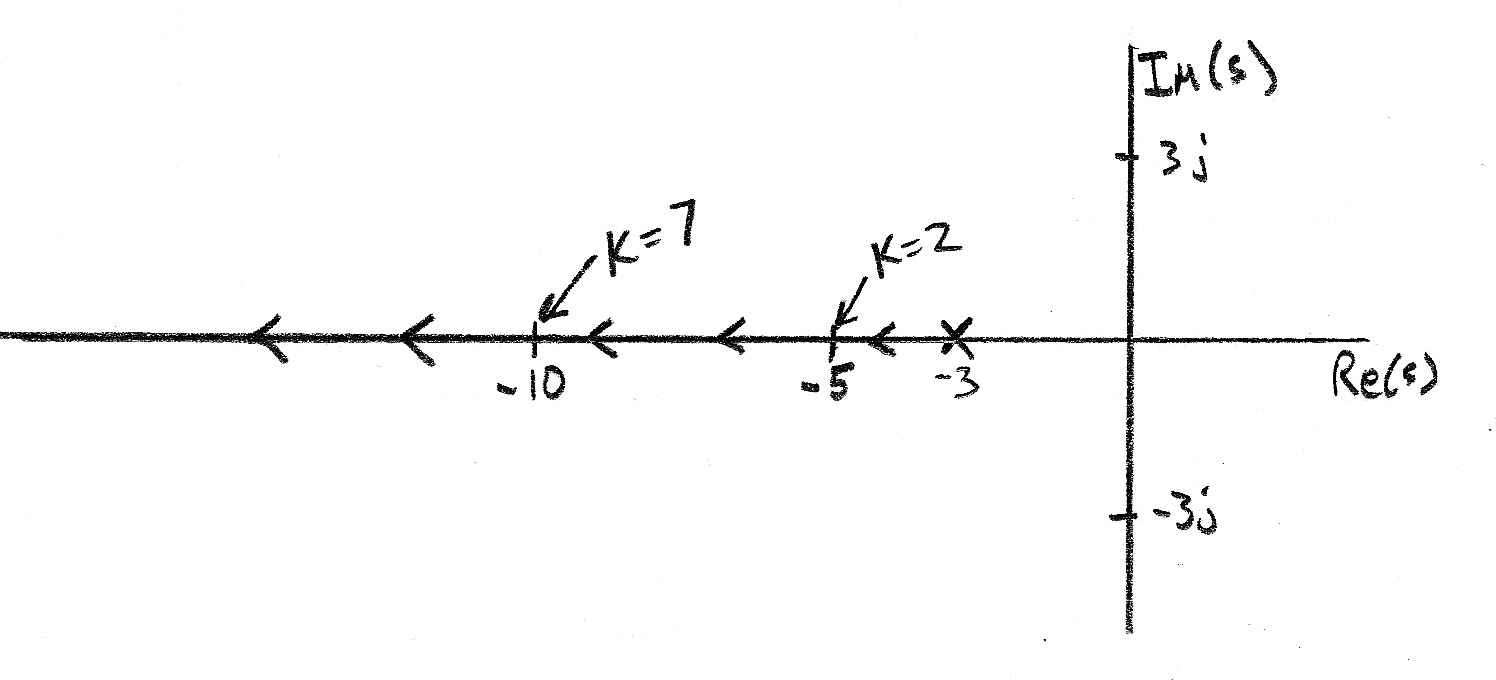
\includegraphics[width=120mm]{figs07/00971.png}
\caption{The closed loop pole of the simple system of Figure \ref{simpleRLsystem} as it moves according to different values of $K$.}\label{movingsimplepole}
\end{figure}




\begin{figure}\centering

%%%%%%%%%%%%%%%%%%%%%%%%%%%%%%%%%%%%%%%%%%%%%%%%%%%%%%%%%%%%%%%%%%%%%%%%%%%%%%%%%%%%%%%%

%        Closed loop control system two blocks / two real OL poles

%%%%%%%%%%%%%%%%%%%%%%%%%%%%%%%%%%%%%%%%%%%%%%%%%%%%%%%%%%%%%%%%%%%%%%%%%%%%%%%%%%%%%%%%

\begin{tikzpicture}[every node/.style={draw, thick,outer sep=0pt,thick}]

% %
% debugging grid
%  \draw[step=5mm,gray,very thin] (-25mm,-25mm) grid (100mm,50mm);
%  \draw[thick,gray] (0,-25mm) -- (0,50mm);
%  \draw[thick,gray] (-25mm,0) -- (100mm,0);
%
%
%
\tikzstyle{init} = [pin edge={to-,thin,black}]


 \node (C) [thick,minimum width=14mm, minimum height=10mm] {$\frac{K(s+1)}{(s+20)}$};

 %plant
 \node (P) [right of=C, node distance=17.5mm,thick,minimum width=14mm, minimum height=10mm] {$\frac{0.2}{(s+2)}$};
 \draw [->] (C.east) -- (P.west);


 % feedback box
 \node (H) [thick, below of=C, xshift=9mm, yshift=-10mm] {$H=1$};

 \coordinate (junct) at ($(C.west)-(5mm,0)$);
 \node (sum)   [circle,draw,minimum width=0.1cm ] at (junct) {};


 % feedback loop
 \coordinate (out1) at ($(P.east)+(5mm,0)$);

 \draw [->]  (out1)   -- (out1 |- H.east) -- (H.east);  % note \- to get x of first and y of second node
 \draw [->] (H.west) --  (sum.south |- H.west) -- (sum.south);

 % controller input
 \draw [->] (sum.east) -- (C.west);

\tikzstyle{every node}=[];

 %error junction and signs
%  \coordinate (junct) at ($(C.west)-(5mm,0)$);
%  \node (sum)   [circle,draw,minimum width=0.1cm ] at (junct) {};
 \node[above left of=sum,xshift=3.5mm,yshift=-3mm](insign){$+$};
 \node[below left of=sum,xshift=4.5mm,yshift=2mm](fbsign){$-$};

 % input
 \draw [<-] (sum.west) -- ++(-3mm,0mm);
 \coordinate  (input) at ($(sum.west)+(-10mm,0)$) node[xshift=-25mm] {$X(s)$};

 % output
 \coordinate (out2)   at ($(P.east)+(10mm,0)$);
 \draw [->] (P.east) -- (out2);
 \node (output) at ($(out2)+(5mm,0mm)$) {$Y(s)$};


% \draw [thick] (Mc.east)  --  (Xa);

\end{tikzpicture}
 \caption{A slightly more complex closed loop control system.}\label{lessSimpleRLsystem}
\end{figure}



But consider a slightly more complex (but still simple) system of Figure \ref{lessSimpleRLsystem}.
Here, the loop gain is obtained by multiplying together the two blocks:
\[
G_L{s} = \frac{0.2K(s+1)}{(s+2)(s+20)}
\]
and it is trivial to see its open loop  poles, but the closed loop gain is
\[
G_{CL}(s) = \frac {0.2K(s+1)} {s^2 + (22+0.2K)s+40+0.2K}
\]
Now as $K$ changes,  it is not at all obvious what are the poles or where they move.  The Root Locus method was invented by Evans to figure this out (without manually solving the denominator polynomials for each value of $K$).


\subsection{Summary}
Some key points about the  Root Locus computation are

\begin{enumerate}
 \item Closed loop poles are not the same as the poles of the individual system blocks.
 \item Closed loop poles predict the time response of closed loop system.
 \item Closed loop poles predict the stability of the closed loop system.
 \item The controller introduces parameter $K$.
 \item The Root Locus diagram is a plot of how closed loop poles change with $K$.
 \item We usually consider $0 \le K \le \infty$.
 \item {\tt python.control} method:  {\tt root_locus_plot(sys) }.
\end{enumerate}



%\end{frame}  %%%%%%%%%%%%%%%%%%%%%%%%%%%%%%%%%%%%%%%%%%%%%%%%%%%%%%%%%%%%

% \vspace{0.0in}  % cleans up line spacing when enumerate breaks into page 97(!!)


%%%%** Section 1.8
\section{Root Locus Examples}



\begin{ExampleSmall}
Use the computer to plot a Root Locus diagram for the system of Section \ref{FeedbackStabilitySection}.
\[
G(s)= CPH(s) = \frac{K}{(s+1)(s+2)(s+3)}
\]


Using python , by default enter the system with $K=1$.:

\begin{verbatim}
  s=ctl.TransferFunction.s
  K = 1
  denom = ((s+1)*(s+2)*(s+3) )
  sys = ctl.TransferFunction(K/denom)
  figRL = plt.Figure()
  ax = plt.gca()
  plt.title("Root Locus Diagram: Example 7.1")
  ctl.root_locus_plot(sys,ax=ax)
  plt.grid()
  plt.show()
\end{verbatim}

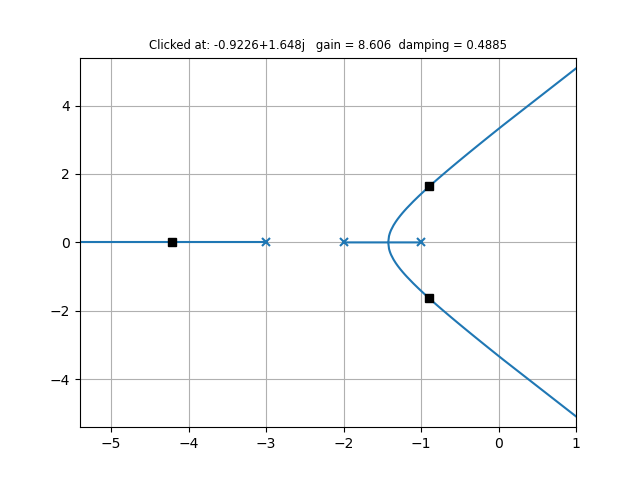
\includegraphics[width=3.5in]{figs07/B47H33.png}

This plot shows first the three ``open loop poles" as X's, all on the negative
real axis.  Lines show the path of the poles as $K\to\infty$. Notice that the
angled lines cross the imaginary axis, at about $\pm3.5j$,
a result consistent with the computation of Section \ref{FeedbackStabilitySection}.
The pole eventually follow straight line asymptotes,
the curved lines (in two cases) are the actual paths. {\bf Note: }
Using {\tt ctl.root_locus_plot()} the lines are clickable!  As shown
I have clicked one of the three black squares  (near $-1+1.6j$),
and the gain value is shown.   Also shown is where the pole at -3 is
for that gain.
\end{ExampleSmall}
\vspace{0.75in}


\begin{ExampleSmall}\label{contplantrootlocus}


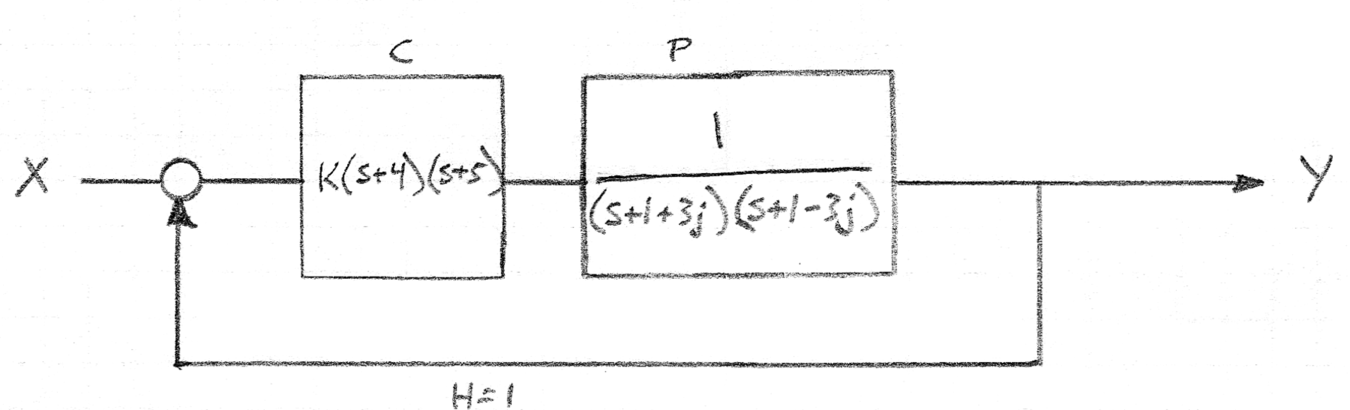
\includegraphics[width=4.5in]{figs07/00780a.png}


Use the computer to plot a Root Locus diagram for the system above.

Here we have two blocks around the loop.  $C$ which represents a controller, and $P$ which represents a plant.  The closed loop system does not care how many blocks are in the loop, just the ``loop gain" which is the product of all blocks around the loop.

\[
G(s) = CPH(s) = C(s)P(s) = \frac {K(s+4)(s+5)}   {(s+1+3j)(s+1-3j)}
\]

\vspace{0.25in}
Using {\tt python.control}:


\begin{verbatim}
  s=ctl.TransferFunction.s
  K =1
  ccp = -1+3j
  ccp2 = -1-3j
  num = K*(s+4)*(s+5)
  denom = ((s-ccp)*(s-ccp2) )
  sys = ctl.TransferFunction(num/denom)
  figRL = plt.Figure()
  ax = plt.gca()
  plt.title("Root Locus Diagram: Example 7.2")
  ctl.root_locus_plot(sys,ax=ax)
  plt.grid()
  plt.show()
\end{verbatim}

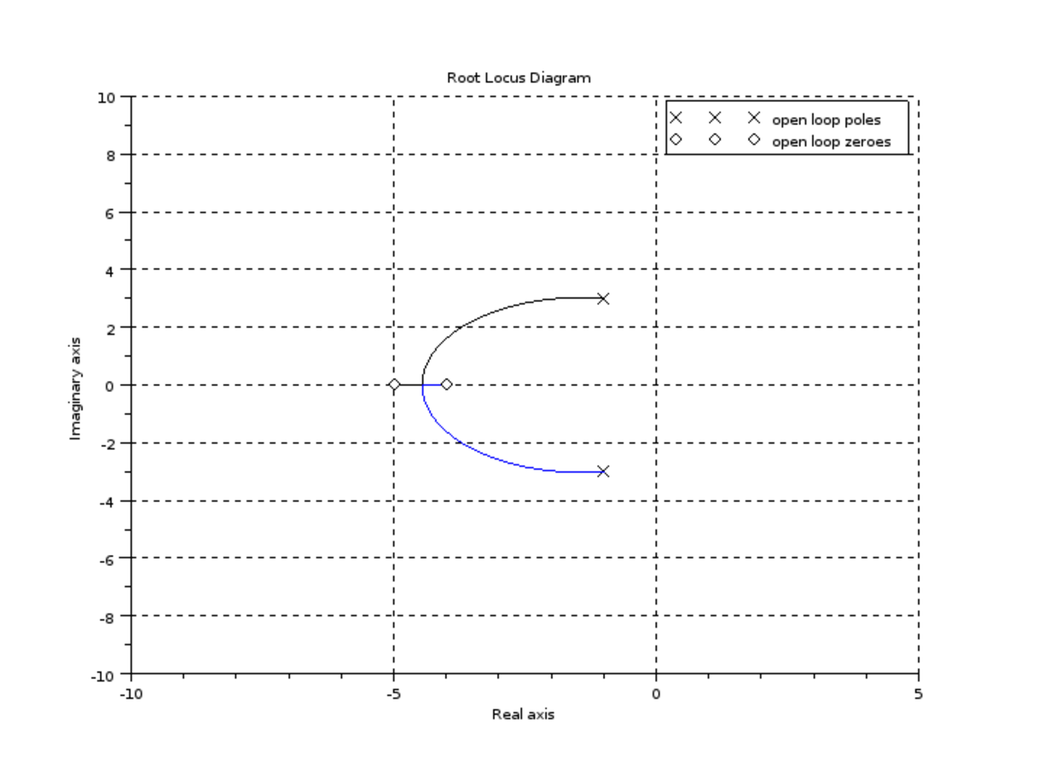
\includegraphics[width=3.5in]{figs07/rlexample2a.png}

This time the closed loop poles migrate toward the two zeros in the controller.  First they leave the loop gain poles (x's) and then join up at the real axis. After that  they split again and migrate along the real axis until they hit the zeros.
\end{ExampleSmall}







%%%%** Section 1.9
\section{Root Locus Steps}

Evans figured out a set of rules, based on the mathematical properties of the closed loop characteristic polynomial, that allow us to sketch the Root Locus diagram quickly.
Recall that the ``loop gain" is the product of all transfer functions around the loop.  For a simple system like that of Example \thechapter.\ref{contplantrootlocus}, the loop gain is $KC(s)P(s)H(s)$ (where we have {\it assumed} that the controller has a constant gain term $K$ and separated it out).  Now we solve the closed loop gain using Equation \ref{hsblackeqn}.
\[
\frac{Y(s)}{X(s)} = \frac  {KC(s)P(s)}   {1+KC(s)P(s)H(s)}
\]
Poles of this closed loop transfer function are values of $s$ where its denominator is zero.  In other words
\[
 {1+KC(s)P(s)H(s)} = 0
\]
giving
\[
{KC(s)P(s)H(s)} = -1
\]
Since the transfer functions are complex, we have
\[
\left | KC(s)P(s)H(s)\right | = 1 \qquad \mathrm{and} \qquad \angle KC(s)P(s)H(s) = 180^\circ
\]
These two conditions are called the {\it magnitude condition} and the {\it angle condition} respectively.
All points on the Root Locus are poles of the closed loop transfer function (CLTF) for different values of $K$.  Since $K$ is positive and real, it always contributes $0^\circ$ to the angle, and can be dropped from the angle condition.  Thus all points on the Root Locus, for any value of $K$ ($0<K<\infty$), must observe both conditions.

The following Root Locus drawing rules derive from either the Magnitude Condition, the Angle Condition, or fundamental properties of polynomials.


%\begin{frame}

{\bf Root Locus (RL) Drawing Steps:}	%<h>
\begin{enumerate}
  \item RL Starts (when $K=0$) at the roots of $CPH(s)$ so start out by  plotting these poles and zeros (as x's and o's).
  \item Find which parts of the real line contain parts of the RL.  For each point on the real axis, if the total number of poles and zeros to right is ODD, that part is ON the RL. Conversely, if the total number of poles and zeros to the right is EVEN, that segment is OFF the RL.
  \item The number of asymptotes (diverging branches which go out to infinity)  is $n_p-n_z$, where $n_p$ is the number of loop gain poles and $n_z$ is the number of zeros.
  \item If $n_p-n_z \neq 0$, the place where the asympototes intersect the real line is:
 $$
 \sigma_a = \frac{\Sigma\mathrm{poles}- \Sigma\mathrm{zeros}}{n_p-n_z}
 $$.

 \item The angles of the diverging branches are:
 $$
 \frac{\pi(1+2m)}{n_p-n_z}
 $$
 where $m$ is the integers $1, 2 , 3, \dots$.
  \item Poles which do NOT diverge circle back to zeros.
\end{enumerate}


%\end{frame}  %%%%%%%%%%%%%%%%%%%%%%%%%%%%%%%%%%%%%%%%%%%%%%%%%%%%%%%%%%%%





%%%%** Section 1.10
\section{Root Locus FAQ}

%\begin{frame}
This FAQ refers to the system of Figure \ref{simpleRLsystem} where $K$ is a real
number $>0$.

\vspace{0.25in}
\begin{quotation}
{\bf Q:}  What is the point of the Root Locus?

{\bf A:}  The point is to predict how {\it closed loop} pole
locations  and  corresponding performance will change as the gain constant, $K$, changes,
knowing only the {\it open loop} poles and zeros.
\end{quotation}

\vspace{0.35in}	%<h>

%\end{frame}  %%%%%%%%%%%%%%%%%%%%%%%%%%%%%%%%%%%%%%%%%%%%%%%%%%%%%%%%%%%%


Each of the following Root Locus Drawing Rules is the answer to a FAQ.

% Make table rows deeper
\renewcommand\arraystretch{2.5}% Vertical Row size, 1.0 is for standard spacing)
\begin{tabular}{p{2.5in}|p{2.5in}|c}
Question			&  Answer			& Reason	\\ \hline \hline
Fact 1. What is true for any value of $s$ on the root locus?
				&  $\angle{CPH(s)} = \pi, 3\pi, 5\pi \dots$, ``Angle Condition" &     \\ \hline
Fact 2. What is $k$ for a value of $s$ on the RL?  &
$|KCPH(s)| = 1$ so $ K = 1/|CPH(s)|$. ``Magnitude Condition"                          &     \\ \hline\hline
Rule 1. Where do branches of the RL go as $k \to \infty$?  &
From poles of $CPH(s)$ to zeros of $CPH(s)$ or they diverge to $|s| = \infty$         & M     \\ \hline
Rule 2. How many branches diverge to  $|s| = \infty$?      &
$n_d = n_p-n_z$.                                                                & P      \\ \hline
Rule 3. What angles do the asymptotes have?                 &
$\theta_d = \frac{\pi(1+2m)}{n_p-n_z},\quad m= 0,1,2,3\dots$                    & A      \\ \hline
Rule 4. Where do asymptotes intersect the real axis?        &
$\sigma_a = \frac{\Sigma\mathrm{poles}- \Sigma\mathrm{zeros}}{n_p-n_z} $        & P      \\ \hline
Rule 5. What parts of the real axis are ON the RL?          &
A segment is ON the RL if the number of real poles and zeros to the right is ODD. & A     \\ \hline \hline
Rule 6. At which point do branches leave or join the real axis?    &
at real values, $s$, where $\frac{d}{ds}\frac{P(s)}{Z(s)}=0$                      & P,A    \\ \hline
Rule 7. At what angle do branches depart from a complex pole? (or join a complex zero?) &
$\theta_d = \pi-\Sigma\angle\mathrm{poles} + \Sigma\angle\mathrm{zeros} $           & A      \\ \hline
\end{tabular}
	%<*>


%\begin{frame}
{\bf Notes:}

Reason codes:
A = ``angle condition", M = ``magnitude condition", P = theory of polynomials.

Rules 6 and 7 are from pre-computer days and no longer needed (in my opinion).













 %%%%%%%%%%%%%%%%%%%%%%%%%%%%%%%%%%%%%%%%%%%%%%%%%%%%%%%%%%%%%%%%%%%%%%%%%%%%%%%%%%%%%%%%%%%%%%%%%%%%%%%%%%%%%%%



\section{Hand Root Locus Examples}

\begin{ExampleSmall}

\begin{tabular}{p{3.0in}p{2.75in}}

\[
G(s) = C(s)P(s) = \frac {K} {(s+5)}
\]

1) Plot the poles and zeros.

2) Real Line: where $Re(s) < -5$ there is one pole to the right.   Therefore RL goes on real line for $x< -5$.

3) \# of diverging asymptotes: $n_p-n_z  = 1-0 = 1  $

4) Angle of Asymptotes:  $\frac{(2m-1)\pi}{n_p-n_z} = \left \{  \pi \right \}$

5) Intercept of asymptotes:  N/A (because $\pi$ is parallel to the real axis).
&
\vtop{\vskip-2ex \hbox{ 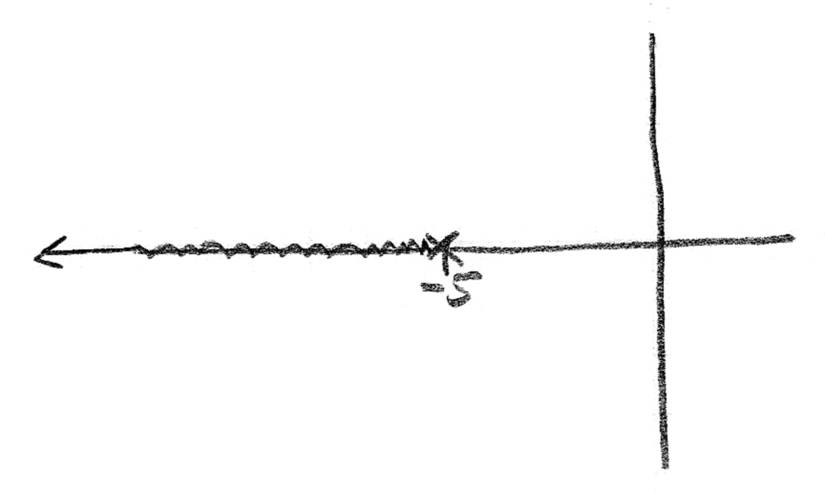
\includegraphics[width=2.75in]{figs07/00783a.png}  }}
\\
\end{tabular}

Interpretation:
As gain $K$ is increased, this system gets more stable and responds faster to input because
$e^{\sigma t}$ gets faster as $\sigma$ gets more negative.

\end{ExampleSmall}

\noindent
\begin{ExampleSmall}

\begin{tabular}{p{3.0in}p{2.75in}}

\[
G(s) = C(s)P(s) = \frac {K} {(s+2)(s+5)}
\]

1) Plot the poles and zeros.

2) Real Line: where $ -5<    Re(s) <  -2$ there is one pole to the right.   Therefore RL goes on real line for $ -5< x < -2$.

3) \# of diverging asymptotes: $n_p-n_z  = 2-0 = 2  $

4) Angle of Asymptotes:  $\frac{(2m-1)\pi}{n_p-n_z} = \left \{  \pi/2 , 3\pi/2 \right \}$

5) Intercept of asymptotes:  $\frac {-2-5} {2} = -3.5$
&
\vtop{\vskip-2ex \hbox{ 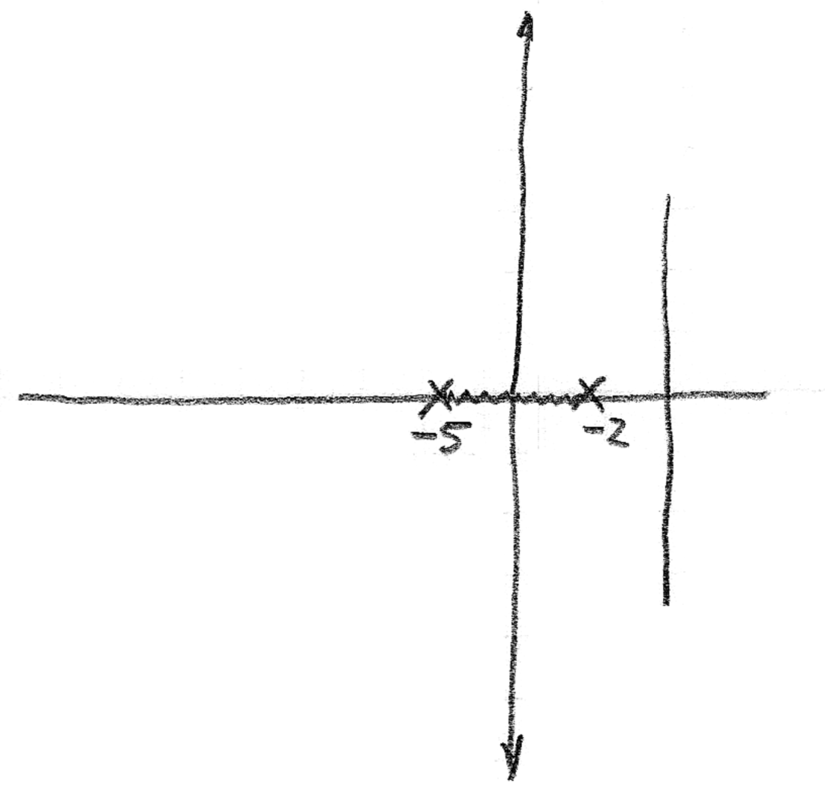
\includegraphics[width=2.75in]{figs07/00784a.png}  }}
\\
\end{tabular}

Interpretation:
After the two closed loop poles meet and diverge along the vertical line at -3.5, they get a bigger and
bigger imaginary component as the gain $K$ increases.   Thus the overshoot in the step response will
increase with gain $K$, and a resonant peak will appear in the frequency response (underdamped response).

\end{ExampleSmall}

\noindent
\begin{ExampleSmall}

\begin{tabular}{p{3.0in}p{2.75in}}

\[
G(s) = C(s)P(s) = \frac {K(s+1)} {(s+2)(s+5)}
\]

1) Plot the poles and zeros.

2) Real Line: where $-2 < Re(s) < -1$ AND $Re(s) < =-5$,  there is an odd number of  poles to the right.

3) \# of diverging asymptotes: $n_p-n_z  = 2-1 = 1  $

4) Angle of Asymptotes:  $\frac{(2m-1)\pi}{n_p-n_z} = \left \{  \pi \right \}$

5) Intercept of asymptotes:  N/A (because $\pi$ is parallel to the real axis).
&
\vtop{\vskip-2ex \hbox{ 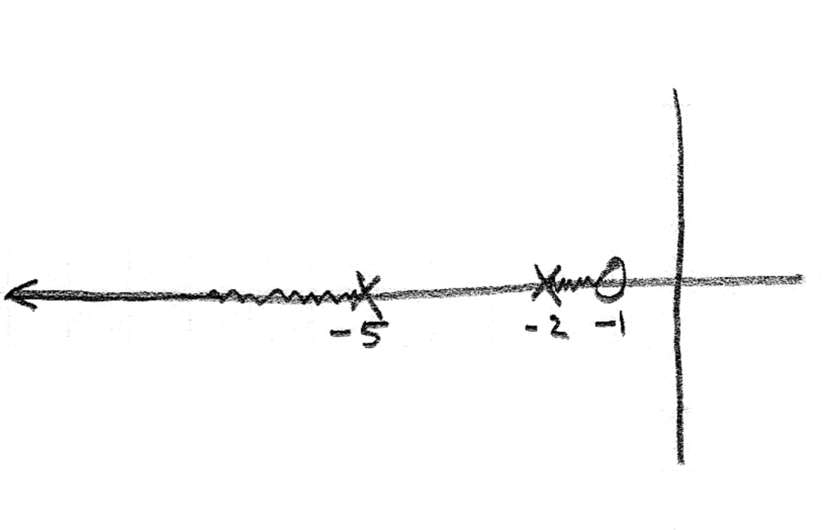
\includegraphics[width=2.75in]{figs07/00785a.png}  }}
\\
\end{tabular}

Interpretation: One pole will get faster as in the first example, but the other pole will converge on
$\sigma = -1$.  Since it is closest to the origin, this pole will dominate the response.   Like the
previous examples, the RL stays in the right half plane and thus is stable for all values of $K>0$.
\end{ExampleSmall}


\noindent
\begin{ExampleSmall}

\begin{tabular}{p{3.0in}p{2.75in}}

\[
G(s) = C(s)P(s) = \frac {K} {(s+5)(s+1+3j)(s+1-3j)}
\]

1) Plot the poles and zeros.

2) Real Line: where $Re(s) < -5$ there are three poles to the right.   Therefore RL goes on real line for $x< -5$.

3) \# of diverging asymptotes: $n_p-n_z  = 3-0 = 3  $

4) Angle of Asymptotes:  $\frac{(2m-1)\pi}{n_p-n_z} = \left \{ \frac{\pi}{3}, \pi , \frac{5\pi}{3}\right \}$

5) Intercept of asymptotes:  $\frac{-5-2}{3} = -2.33$.
&
\vtop{\vskip-2ex \hbox{ 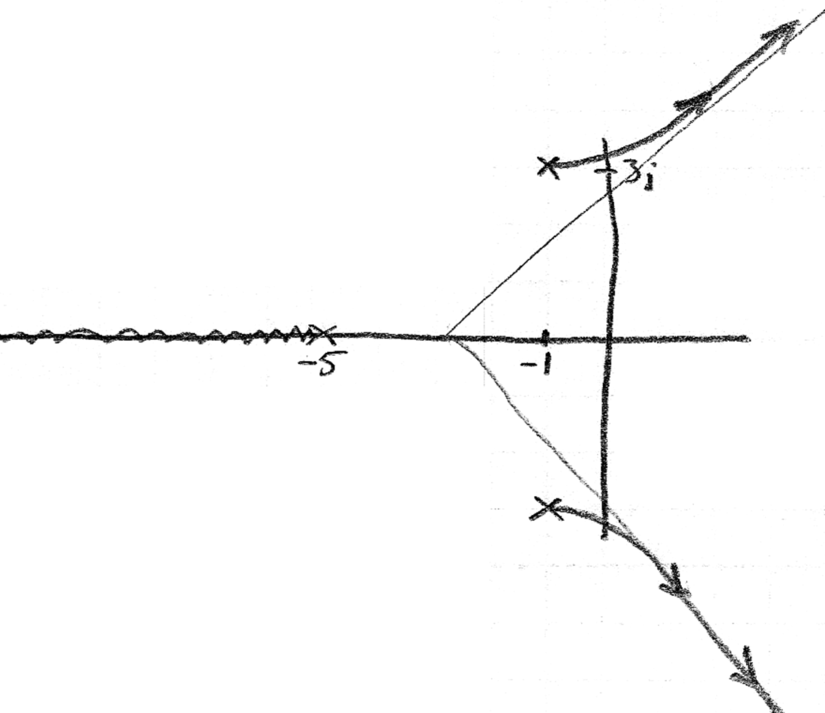
\includegraphics[width=2.75in]{figs07/00781a.png}  }}\\
\end{tabular}

Interpretation: The two complex conjugate poles cross into the right hand side ($Re(s) > 0$) at some value of $K$.
This system will thus go unstable for $K> x$ (we will see how to find $x$ later).
\end{ExampleSmall}



\noindent
\begin{ExampleSmall}

\begin{tabular}{p{3.0in}p{2.75in}}

\[
G(s) = C(s)P(s) = \frac {K(s+4)} {(s+5)(s+1+3j)(s+1-3j)}
\]

1) Plot the poles and zeros

2) Real Line: $-5< Re(s) < -4$

3) \# of diverging asymptotes: $n_p-n_z =3-1 =2   $

4) Angle of Asymptotes:  $\frac{(2m-1)\pi}{2} = \left \{ \pi/2, 3\pi/2 \right \}$

5) Intercept of asymptotes:  $\frac {-5-2+4}{3-1} = -1.5$
&
\vtop{\vskip-2ex \hbox{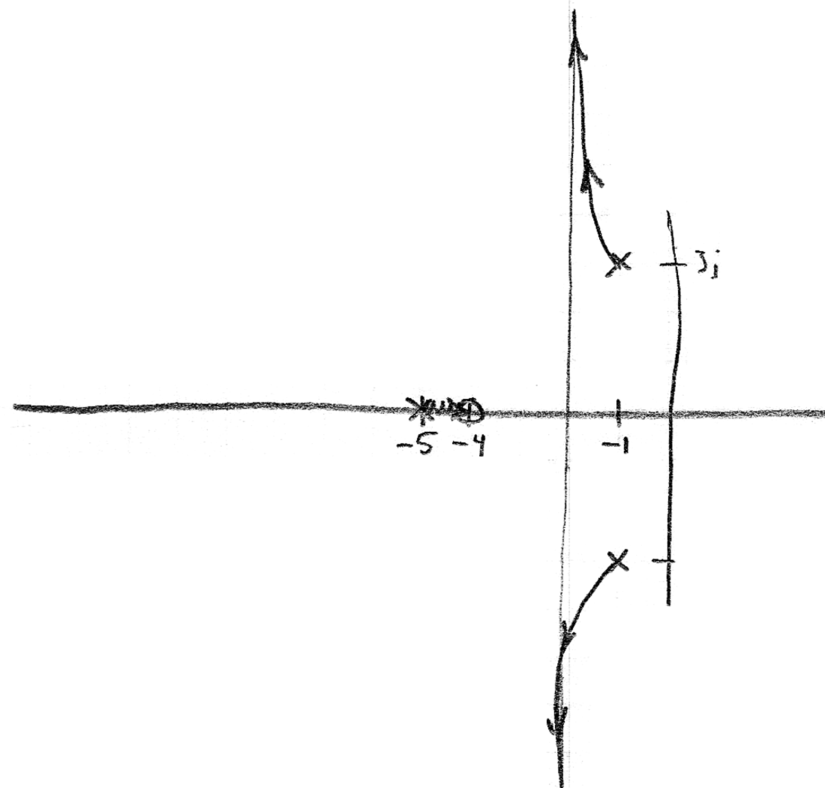
\includegraphics[width=2.75in]{figs07/00782a.png} }} \\
\end{tabular}

Interpretation:  This is the same system as the previous example, except we added a zero at
$s=-4$.   Note how the RL now stays entirely in the left half plane.  The system is now
stable for all values of $K>0$.
\end{ExampleSmall}


\noindent
\begin{ExampleSmall}

\begin{tabular}{p{3.0in}p{2.75in}}
\[
G(s) = C(s)P(s) = \frac {K(s+4)(s+5)} {(s+1+3j)(s+1-3j)}
\]

1) Plot the poles and zeros

2) Real Line: $-5<Re(s)< -4$

3) \# of diverging asymptotes: $n_p-n_z = 0    $

4) Angle of Asymptotes:  N/A (because no asymptotes)

5) Intercept of asymptotes:  N/A

&
\vtop{\vskip-2ex \hbox{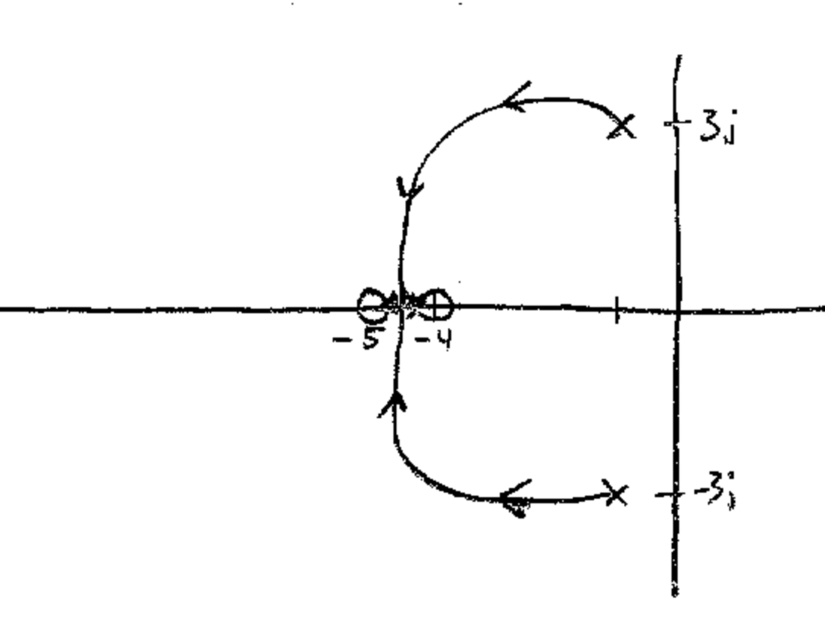
\includegraphics[width=2.75in]{figs07/00474a.png} }} \\
\end{tabular}

Interpretation: Adding a second zero ``pulls" the RL even more to the left --- makes it even more
stable.

(Compare to Example \thechapter.\ref{contplantrootlocus}).
\end{ExampleSmall}


%%%%%%%%%%%%%%%%%%%%%%%%%%%%%%%%%%%%%%%%%%%%%%%%%%%%%%%%%%%%%%%%%%%%%%%%%%%%%%%%%%%%%%%%%%%%%%%
\section{Resources}
A very nice web resource on the Root Locus:

\url{http://lpsa.swarthmore.edu/Root_Locus/RootLocusReviewRules.html}

% \section{Summary of Notation}

